%%%
% Plantilla de Memoria
% Modificación de una plantilla de Latex de Nicolas Diaz para adaptarla 
% al castellano y a las necesidades de escribir informática y matemáticas.
%
% Editada por: Mario Román
%
% License:
% CC BY-NC-SA 3.0 (http://creativecommons.org/licenses/by-nc-sa/3.0/)
%%%

%%%%%%%%%%%%%%%%%%%%%%%%%%%%%%%%%%%%%%%%%
% Thin Sectioned Essay
% LaTeX Template
% Version 1.0 (3/8/13)
%
% This template has been downloaded from:
% http://www.LaTeXTemplates.com
%
% Original Author:
% Nicolas Diaz (nsdiaz@uc.cl) with extensive modifications by:
% Vel (vel@latextemplates.com)
%
% License:
% CC BY-NC-SA 3.0 (http://creativecommons.org/licenses/by-nc-sa/3.0/)
%
%%%%%%%%%%%%%%%%%%%%%%%%%%%%%%%%%%%%%%%%%

%----------------------------------------------------------------------------------------
%	PAQUETES Y CONFIGURACIÓN DEL DOCUMENTO
%----------------------------------------------------------------------------------------

%%% Configuración del papel.
% microtype: Tipografía.
% mathpazo: Usa la fuente Palatino.
\documentclass[a4paper, 20pt]{article}
\usepackage[a4paper,margin=1in]{geometry}
\usepackage[protrusion=true,expansion=true]{microtype}
\usepackage{mathpazo}

% Indentación de párrafos para Palatino
\setlength{\parindent}{0pt}
  \parskip=8pt
\linespread{1.05} % Change line spacing here, Palatino benefits from a slight increase by default


%%% Castellano.
% noquoting: Permite uso de comillas no españolas.
% lcroman: Permite la enumeración con numerales romanos en minúscula.
% fontenc: Usa la fuente completa para que pueda copiarse correctamente del pdf.
\usepackage[spanish,es-noquoting,es-lcroman,es-tabla,,es-nodecimaldot]{babel}
\usepackage[utf8]{inputenc}
\usepackage{fontenc}
\selectlanguage{spanish}

%%% Matemáticas
\usepackage{amsmath}

%%% Gráficos
\usepackage{graphicx} % Required for including pictures
\usepackage{wrapfig} % Allows in-line images
\graphicspath{{./fig/}}
\usepackage[usexcolor=false, inkscape=true]{svg} % Required for including svg
\svgpath{{./fig/}}
\usepackage[usenames,dvipsnames]{color} % Coloring code



%%% Pseudocódigo
\usepackage{algorithmicx}
\usepackage[ruled]{algorithm}
\usepackage{algpseudocode}

\newcommand{\alg}{\texttt{algorithmicx}}
\newcommand{\old}{\texttt{algorithmic}}
\newcommand{\euk}{Euclid}
\newcommand\ASTART{\bigskip\noindent\begin{minipage}[b]{0.5\linewidth}}
\newcommand\ACONTINUE{\end{minipage}\begin{minipage}[b]{0.5\linewidth}}
\newcommand\AENDSKIP{\end{minipage}\bigskip}
\newcommand\AEND{\end{minipage}}

%%% Código
\usepackage{listings}

%%% Tablas
\usepackage{tabularx}
\usepackage{float}
\usepackage{adjustbox}
\usepackage{booktabs}
\usepackage{array}
\newcolumntype{L}[1]{>{\raggedright\let\newline\\\arraybackslash\hspace{0pt}}m{#1}}
\newcolumntype{C}[1]{>{\centering\let\newline\\\arraybackslash\hspace{0pt}}m{#1}}
\newcolumntype{R}[1]{>{\raggedleft\let\newline\\\arraybackslash\hspace{0pt}}m{#1}}

% Enlaces y colores
\usepackage{hyperref}
\usepackage[dvipsnames]{xcolor}
\definecolor{webgreen}{rgb}{0,0.5,0}
\hypersetup{
  colorlinks=true,
  citecolor=RoyalBlue,
  urlcolor=RoyalBlue,
  linkcolor=RoyalBlue
}

%%% Bibliografía
\usepackage[backend=biber]{biblatex}
\DefineBibliographyStrings{spanish}{
  urlseen = {Último acceso}
}
\addbibresource{IN-P2.bib}

%----------------------------------------------------------------------------------------
%	TÍTULO
%----------------------------------------------------------------------------------------
% Configuraciones para el título.
% El título no debe editarse aquí.
\renewcommand{\maketitle}{
  \begin{flushright} % Right align
  
  {\LARGE\@title} % Increase the font size of the title
  
  \vspace{50pt} % Some vertical space between the title and author name
  
  {\large\@author} % Author name
  \\\@date % Date
  \vspace{40pt} % Some vertical space between the author block and abstract
  \end{flushright}
}

%% Título
\title{\textbf{Título}\\ % Title
Subtítulo} % Subtitle

\author{\textsc{Autor1,\\Autor2} % Author
\\{\textit{Universidad de Granada}}} % Institution

\date{\today} % Date

%-----------------------------------------------------------------------------------------
%	DOCUMENTO
%-----------------------------------------------------------------------------------------

\begin{document}

%-----------------------------------------------------------------------------------------
%	TITLE PAGE
%-----------------------------------------------------------------------------------------

\begin{titlepage} % Suppresses displaying the page number on the title page and the subsequent page counts as page 1
	
	\raggedleft % Right align the title page
	
	\rule{1pt}{\textheight} % Vertical line
	\hspace{0.05\textwidth} % Whitespace between the vertical line and title page text
	\parbox[b]{0.8\textwidth}{ % Paragraph box for holding the title page text, adjust the width to move the title page left or right on the page
		
		{\Huge\bfseries Práctica 3:\\[0.5\baselineskip] Competición en DrivenData}\\[2\baselineskip] % Title
		{\large\textit{Curso 2019/2020}}\\[4\baselineskip] % Subtitle or further description
		{\Large\textsc{Sofía Almeida Bruno}\\[0.5\baselineskip]sofialmeida@correo.ugr.es} % Author name, lower case for consistent small caps
		
		\vspace{0.4\textheight} % Whitespace between the title block and the publisher
		
		{\noindent Grupo IN 2\\[0.5\baselineskip] Jueves 9:30-10:30}\\[\baselineskip] % Publisher and logo
	}

\end{titlepage}

%% Resumen (Descomentar para usarlo)
%\renewcommand{\abstractname}{Resumen} % Uncomment to change the name of the abstract to something else
%\begin{abstract}
% Resumen aquí
%\end{abstract}

%% Palabras clave
%\hspace*{3,6mm}\textit{Keywords:} lorem , ipsum , dolor , sit amet , lectus % Keywords
%\vspace{30pt} % Some vertical space between the abstract and first section


%% Índice
{\parskip=2pt
  \tableofcontents
}
\pagebreak

%%%%%%%%%%%%%%%%%%%%%%%%%%%%%%%%%%%%%%%%%%%%%%%%%%%%%%%%%%%%%%%%%%%
%       Captura de pantalla de Submissions
%%%%%%%%%%%%%%%%%%%%%%%%%%%%%%%%%%%%%%%%%%%%%%%%%%%%%%%%%%%%%%%%%%%
\section{Captura de pantalla de Submissions}
\label{sec:subsimissions}
\pagebreak

%%% Inicio del documento
%%%%%%%%%%%%%%%%%%%%%%%%%%%%%%%%%%%%%%%%%%%%%%%%%%%%%%%%%%%%%%%%%%%
%       DESCRIPCIÓN DEL PROBLEMA
%%%%%%%%%%%%%%%%%%%%%%%%%%%%%%%%%%%%%%%%%%%%%%%%%%%%%%%%%%%%%%%%%%%
\section{Introducción}


%%% Inicio del documento
%%%%%%%%%%%%%%%%%%%%%%%%%%%%%%%%%%%%%%%%%%%%%%%%%%%%%%%%%%%%%%%%%%%
%       Pruebas realizadas
%%%%%%%%%%%%%%%%%%%%%%%%%%%%%%%%%%%%%%%%%%%%%%%%%%%%%%%%%%%%%%%%%%%
\section{Pruebas realizadas}
\begin{table}[H]
\centering
\caption{Pruebas realizadas}
\label{tab:pruebas}
\makebox[\textwidth][c]{\begin{tabular}{lL{2cm}lllL{3cm}L{2.5cm}L{3.5cm}}
\toprule
ID & Fecha-hora & Pos. & Sc.-Training & Sc.-Test & Preprocesado & Algoritmos & Parámetros\\
\midrule
00 & 5/12/2019 10:07:58 UTC & 315 & 0.7264 & 0.6883 & ESTO ES UN PRUEBA DE ESCRIBIR MUCHAS CMUCHAS MUCHAS COSAS QUE VOY A HACER PARA PREPROCESAR & Lightgbm & {\ttfamily objective = 'regression\_l1', n\_estimators = 200, n\_jobs = 2}\\

01 & 19/12/2019 11:18:10 UTC & 356 & 0.7358 & 0.6874 & - & Lightgbm & {\ttfamily objective = 'regression\_l1', n\_estimators = 200, n\_jobs = 2, feature\_fraction = 0.5, learning\_rate = 0.1, num\_leaves = 50}\\
\bottomrule
\end{tabular}}
\end{table}
\newpage

\section{Diario de pruebas}
\subsection{\texttt{p3\_00}}
Comenzamos aprendiendo a subir los resultados de test a la plataforma para que puedan ser validados. El script utilizado en esta ocasión es el proporcionado por el profesor de la asignatura. No se realiza ningún preprocesado y el algoritmo a utilizar es Lightgbm un algoritmo de boosting.
%TODO: Comentar algo de lightgbm vs xgboost

\subsection{\texttt{p3\_01}}
\subsubsection{Análisis exploratorio de los datos}

Antes de decidir qué hacer a continuación debemos conocer cierta información sobre los datos. Podemos pensar que necesitamos algún tipo de preprocesado, pues es lo habitual en este tipo de problema, pero sin conocer exactamente cómo son nuestros datos, si tienen o no ruido, la cantidad de valores perdidos, correlación entre las variables, \dots no podremos decidir cómo enfocar el preprocesado ni qué necesidades tiene el conjunto. Para ello comenzamos a escribir algunas funciones de visualización que nos permitan conocer esta información, se encuentran en el \textit{script} \texttt{visualization.py}

Inspirándonos en 
https://www.kaggle.com/kerneler/starter-richter-s-predictor-modeling-e7f51e9e-e
observamos en la Figura \ref{fig:tam_clases} la distribución de las clases.

\begin{figure}[H]
    \centering
    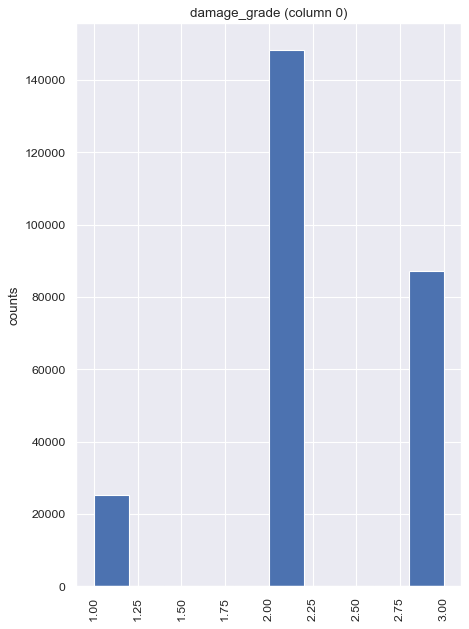
\includegraphics[height=0.6\textwidth, width=0.6\textwidth]{260601_dist}
    \caption{Tamaño de las clases}
    \label{fig:tam_clases}
\end{figure}

Nuestras clases están claramente desbalanceadas, en la Tabla \ref{tab:tam_clas} observamos con exactitud el número de ejemplos que tenemos de cada clase. Ante esta situación se nos ocurren dos opciones: elegir un algoritmo que esté diseñado para manejar esta situación, utilizar técnicas específicas para paliarlo.

% Tabla tamaño de clases
\begin{table}[H]
\centering
\caption{Tamaño de las clases}
\label{tab:tam_clas}
\begin{tabular}{lrr}
\toprule
Clase & Número de elementos & Tamaño de la clase\\
\midrule
1 & 25124 & 9.64\%\\
2 & 148259 & 56.89\%\\
3 & 87218 & 33.47\%\\
\bottomrule
\end{tabular}
\end{table}

También podemos observar la correlación entre las variables en la Figura \ref{fig:corr_matrix}.


\begin{figure}[H]
  \centering
  \includesvg[height=1\textwidth, width=1\textwidth]{corr_matrix}
  \caption{Matriz de correlación}
  \label{fig:corr_matrix}
\end{figure}


% A partir de aquí la inspiración viene de...
% https://www.kaggle.com/jaylaksh94/model-for-nepal-earthquake-damage
Mediante \texttt{data\_x.info()} conocemos que de las 38 variables 30 son numéricas y 8 categóricas, accedemos a la descripción del problema en %https://www.drivendata.org/competitions/57/nepal-earthquake/page/136/
para conocer cuántos posibles valores toman las variables categóricas. Toman entre 3 y 10 posibles valores. En esta página también nos percatamos de que, de las variables numéricas, muchas son de tipo binario.

Ejecutando \texttt{data\_x.isnull().any()} nos damos cuenta de que nuestras variables no contienen valores perdidos, podemos ahorrarnos la imputación de valores perdidos.

% TODO: Ver si hay ruido

\subsubsection{Ajuste de Lightgbm}

Para tratar de conseguir mejores resultados tenemos, a priori, dos caminos: preprocesar los datos, mejorar el algoritmo. Para mejorar el algoritmo hay, a su vez, dos opciones: elegir el algoritmo y ajustar sus parámetros.

En primer lugar trataremos de ajustar los parámetros de Lightgbm a ver si mejora el resultado. Usando el código de ejemplo \texttt{ejemplo\_ds\_avanzado} nos centraremos en los parámetros \texttt{feature\_fraction} (que tomará ..., \texttt{learning\_rate}, \texttt{num\_leaves}. Fijando \texttt{n\_estimators = 200}. Tras realizar el \texttt{GridSearch} se obtiene (tras 10 minutos de ejecución) que los mejores parámetros son: \texttt{feature\_fraction = 0.5}, \texttt{learning\_rate = 0.1},  \texttt{n\_estimators = 200}, \texttt{num\_leaves = 50}.

Obtenemos un resultado en training de 0.7358 y en test de 0.6874, disminuyendo con respecto al anterior envío, a pesar de haber aumentado en test. ¿Se está produciendo sobre ajuste?

\subsection{\texttt{p3\_02}}

%% Comprobamos qué ocurre si nos quedamos con menor \texttt{learning\_rate}. Usamos los parámetros ajustados, modificando solo la variable comentada. Los parámetros utilizados son: \texttt{feature\_fraction = 0.5}, \texttt{learning\_rate = 0.05},  \texttt{n\_estimators = 200}, \texttt{num\_leaves = 50}.
Nos preguntamos qué está provocando este sobreajuste, así comprobamos los valores de las variables por defecto y los utilizados. El que más se diferencia es \texttt{num\_leaves}, por defecto es 31 y estamos tomando 50. Realizaremos un GridSearch
objetivo: menor número de hojas con mejor resultado.
\subsection{\texttt{p3\_03}}
%https://lightgbm.readthedocs.io/en/latest/Parameters.html#weight_column
Tras observar los parámetros de Lightgbm nos damos cuenta de que tiene una opción en la que el propio algoritmo trata este tipo de variables

% TODO:
% - Pasar a textit: script, test, training, boosting
% TODO:
% - Referenciar referencias...
%%%%%%%%%%%%%%%%%%%%%%%%%%%%%%%%%%%%%%%%%%%%%%%%%%%%%%%%%%%%%%%%%%%
%       REFERENCIAS
%%%%%%%%%%%%%%%%%%%%%%%%%%%%%%%%%%%%%%%%%%%%%%%%%%%%%%%%%%%%%%%%%%%
\printbibliography
\end{document}
